\section{Cloud Computing}

\textbf{Cloud computing is a form of distributed computing that turns compute infrastructure, programming
platforms and software systems into scalable utility services~\cite{hassan2011demystifying,Mell:2011:SND:2206223}.}
By exposing various compute and programming
resources as utility services, cloud computing promotes resource sharing at scale via the Internet.
The cloud model precludes the users from having to set up their own hardware, and in some cases also software. Instead,
the users can simply acquire the resources ``in the cloud'' via the internet, and relinquish them when
the resources are no longer needed. The cloud model also does not require the users to spend any start up
capital. The users only have to pay for the resources they acquired, usually based on a pay-per-use
billing model.

\textbf{Depending on the type of resources
offered as services, cloud computing platforms can be categorized into three main categories~\cite{Mell:2011:SND:2206223}.}
\begin{description}
\item [Infrastructure-as-a-Service clouds (IaaS)]
Offers low-level compute, storage and networking
resources as a service. Compute resources are typically provided in the form of on-demand virtual machines (VMs)
with specific CPU, memory and disk configurations (e.g. Amazon EC2, Google Compute Engine, Eucalyptus). 
The provisioned VMs usually come with a base operating system installed. The users must install all the application software
necessary to use them.
\item [Platform-as-a-Service clouds (PaaS)]
Offers a programming platform as a service, that can be used to develop and deploy applications at scale 
(e.g. Google App Engine, AppScale, Heroku, Amazon Elastic Beanstalk). The programming platform consists
of several scalable services that can be used to obtain certain application features such as data storage, caching
and authentication.
\item [Software-as-a-Service clouds (SaaS)]
Offers a collection of software applications and tools as a service, that can be directly consumed by
application endusers (e.g. Salesforce, Workday, Citrix go2meeting). This can be thought of as a new way 
of delivering software to
endusers. Instead of prompting the users to download and install any software, SaaS enables the users
to consume software via the Internet.  
\end{description}

Due to these benefits associated with cloud computing (scalability, high availability, productivity enhancement etc.),
many developers and organizations use the cloud as their preferred means of developing and deploying
software applications. \textbf{Cloud-hosted applications expose one or more web application programming 
interfaces (web APIs) through which client programs can remotely interact with the applications.} That is, clients
send HTTP/S requests to the API, and receive machine readable responses (e.g. HTML, JSON,
XML, Protocol Buffers~\cite{protobuff}) in return. This type of web-accessible, cloud-hosted applications
tend to be highly interactive, and clients have strict expectations on the application
response time~\cite{latency-matters}.

\textbf{A cloud-hosted application may
also consume web APIs exposed by other cloud-hosted applications.} Thus, cloud-hosted applications
form an intricate graph of inter-dependencies among them, where each application can service a set of client
applications, while being dependent on a set of other applications. However, in general, each cloud-hosted
application directly depends on the core services offered by the underlying cloud platform for compute power, storage,
network connectivity and scalability.

In the next section we take a closer look at a specific type of cloud platforms -- Platform-as-a-Service clouds.
We use PaaS clouds as a case study and a testbed in a number of our explorations.

\section{Platform-as-a-Service Clouds}

\textbf{PaaS clouds, which have been growing in popularity~\cite{paas-growth,paas-growth2}, 
typically host web-accessible (HTTP/S) applications, to which they provide
high levels of scalability, availability, and sandboxed execution.} PaaS clouds
provide scalability by automatically allocating resources for
applications on the fly (auto scaling), and provide availability through the
execution of multiple instances of the application. Applications deployed on
a PaaS cloud depend on a number of scalable services intrinsic to the 
cloud platform. We refer to these services as \textit{kernel services}.

\textbf{PaaS clouds, through their kernel services, provide a high level of
abstraction to the application developer that effectively hides all the
infra\-structure-level details such as physical resource allocation (CPU,
memory, disk etc), operating system, and network configuration.} 
Moreover, PaaS clouds do not require the developers
to set up any utility services their applications might require such as a 
database or a distributed cache. 
Everything an application requires is provisioned and managed by the PaaS cloud.
This enables
application developers to focus solely on the programming aspects of their
applications, without having to be concerned about deployment issues. On
the other hand, the software abstractions provided by PaaS clouds obscure
runtime details of applications making it difficult to reason about application
performance, and diagnose performance issues.

\begin{figure}
\centering
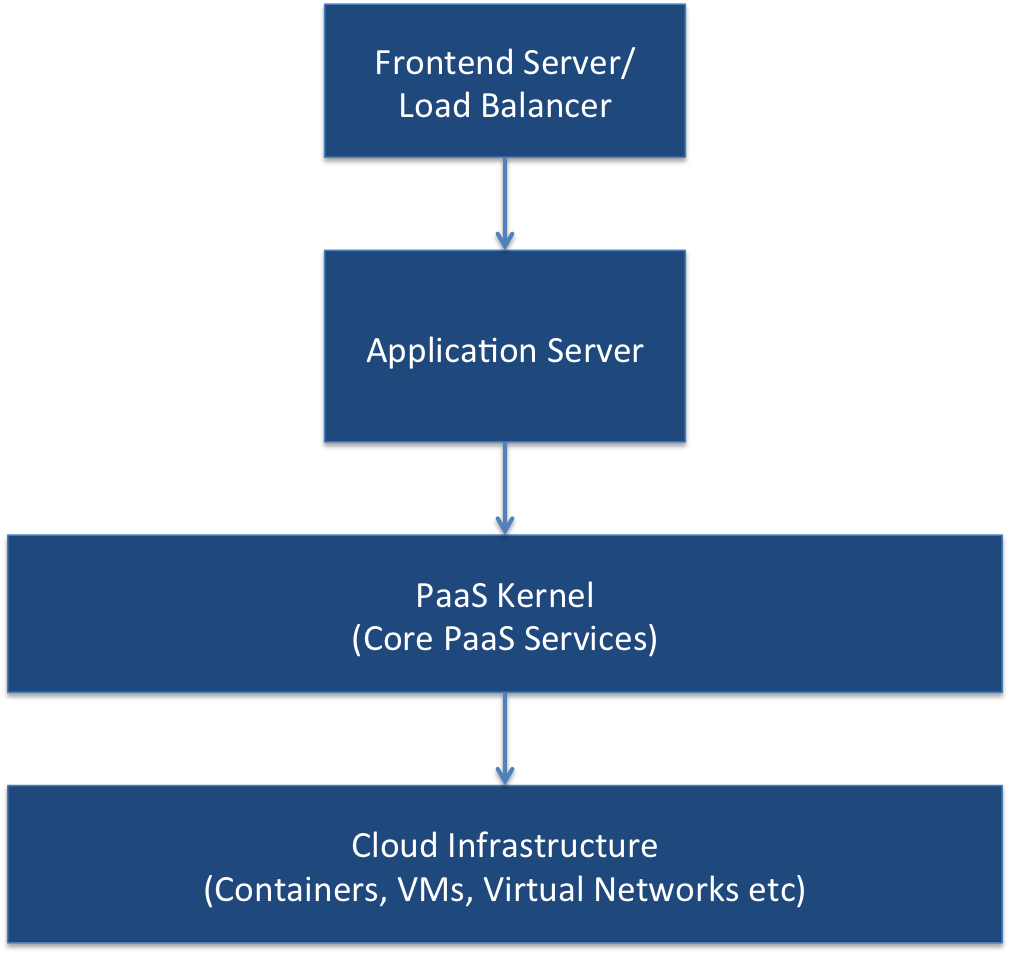
\includegraphics[scale=0.5]{paas_architecture}
\caption{PaaS system organization.}
\label{fig:paas_architecture}
\end{figure}

Figure~\ref{fig:paas_architecture} shows the key layers of a typical PaaS cloud. Arrows indicate
the flow of data and control in response to application requests.
\textbf{At the lowest level of a PaaS cloud is an infrastructure that consists of the necessary compute, storage
and networking resources.} How this infrastructure is set up may vary from a simple cluster of physical 
machines to a comprehensive Infrastructure-as-a-Service (IaaS) cloud. In large scale PaaS clouds,
this layer typically consists of many virtual machines and/or containers with the ability to acquire more
resources on the fly.

\textbf{On top of the infrastructure layer lies the PaaS kernel -- a collection of managed, scalable
services that high-level application developers can compose into their applications.} The provided kernel services
may include database services, caching services, queuing services and more. 
The implementations of the kernel services are highly scalable, highly available (have SLOs associated with them),
and automatically managed by the platform while being completely opaque
to the application developers. Some PaaS clouds
also provide a managed set of programming APIs (a ``software development
kit'' or SDK) for the application developer to access these kernel services. 
In that case all interactions between the applications and the PaaS kernel must take place through
the cloud provider specified SDK (e.g. Google App Engine~\cite{gae}, Microsoft Azure~\cite{azure}). 

\textbf{One level above the PaaS kernel we find the application servers that are used to deploy and run
applications.} Application servers provide the necessary integration (linkage) between application code and the
PaaS kernel services, while sandboxing application code for secure, multi-tenant execution. They also
enable horizontal scaling of applications by running the same application on multiple application server
instances.

\textbf{On top of the application servers layer resides the request
front-end and load balancing layer.} This layer is responsible
for receiving all application requests, filtering them, and routing them to an appropriate application
server instance for further execution. Front-end server is therefore the entry point for PaaS-hosted
applications for all application clients.

\textbf{Each of the above layers can span multiple processes, running over multiple physical or virtual
machines.} Therefore processing a single application request typically involves cooperation
of multiple distributed processes and/or machines.

\begin{figure}
\centering
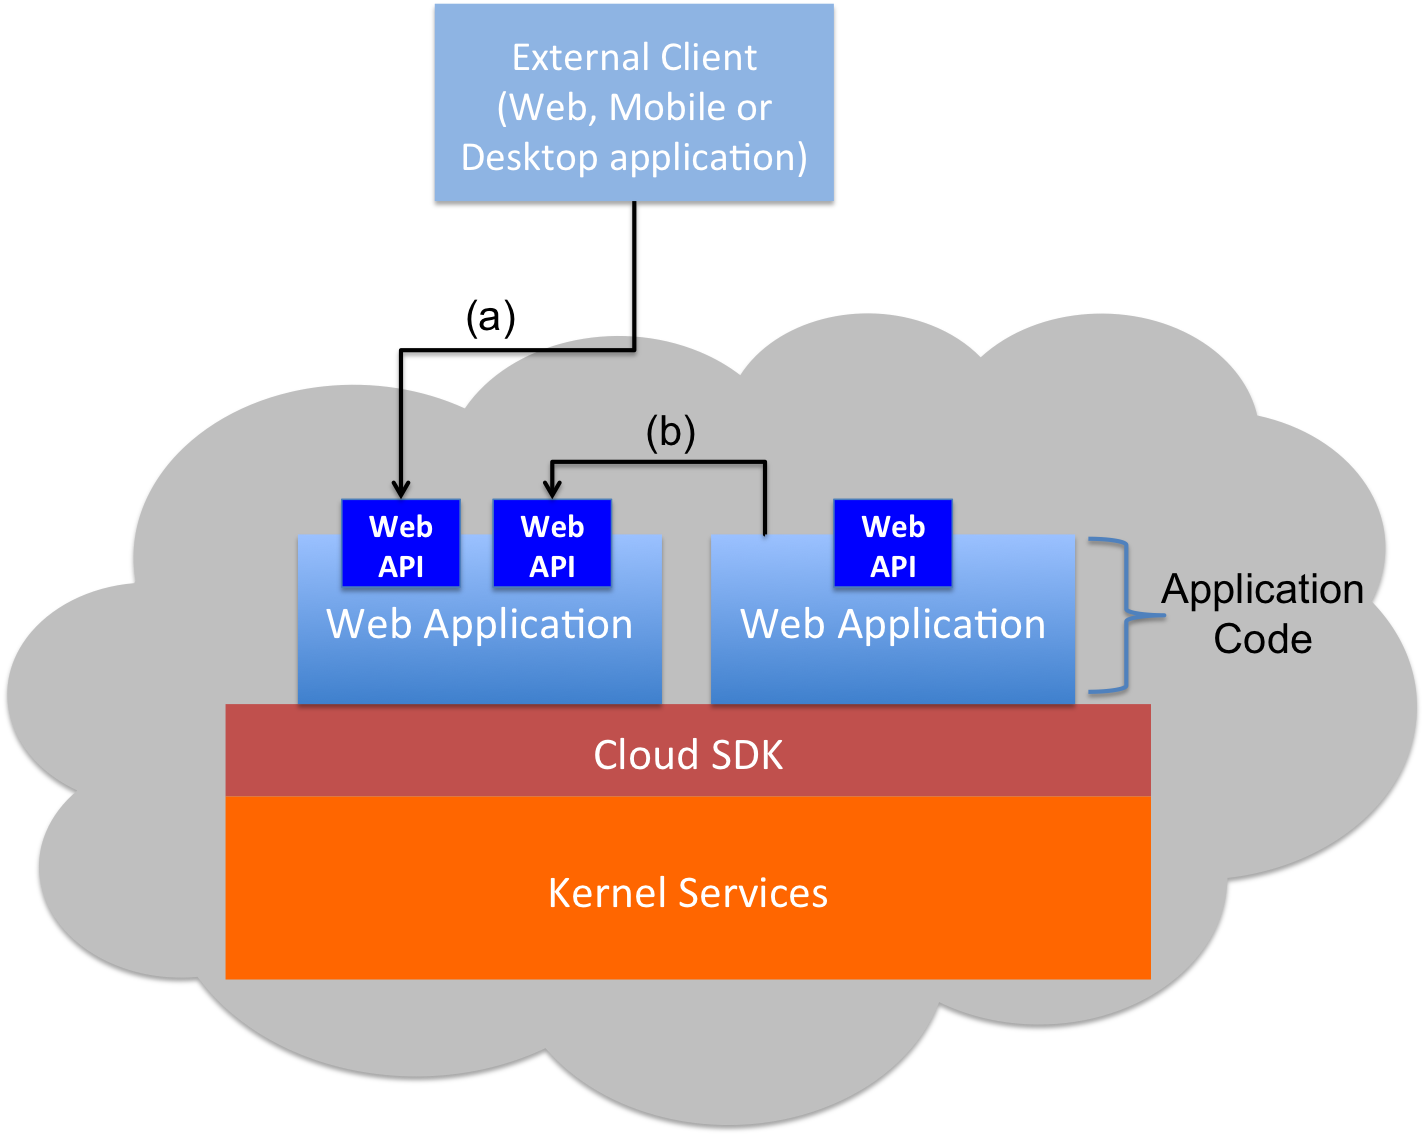
\includegraphics[scale=0.4]{cloud_app_model2}
\caption{Applications deployed in a PaaS cloud: (a) An external client making requests
to an application via the web API;
(b) A PaaS-hosted application invoking another in the same cloud.
\label{fig:cloud_app_model}
}
\end{figure}

Figure~\ref{fig:cloud_app_model} illustrates the application deployment model of PaaS clouds. 
The cloud platform provides a set of kernel services. 
The PaaS SDK provides well defined interfaces (entry points) for these kernel services.  
\textbf{The developer uses the kernel services, via the SDK, to implement his/her application logic, and packages 
it as a web application.} Developers then
upload their applications to the cloud for deployment.
Once deployed, the applications and any web APIs exported by them can be accessed 
via HTTP/S requests by external or co-located clients.

\textbf{PaaS clouds are specifically built for deploying and running applications
that are directly consumed by end users and other client applications.} As a result all the problems 
outlined in the previous chapter, such as poor development practices, lack of performance SLOs, and lack of performance 
debugging support directly impact PaaS clouds. Therefore PaaS clouds are ideal candidates for implementing the type
of governance systems proposed in this work. 

\textbf{We use PaaS clouds in our research extensively both as case studies
and experimental platforms.} Specifically, we use Google App Engine and AppScale as test environments
to experiment with our new governance systems. App Engine is a highly scalable public PaaS cloud hosted and
managed by Google in their data centers. While it is open for anyone to deploy and run web applications, it is not
open source software, and its internal deployment details are not commonly known. AppScale is open source
software that can be used to set up a private cloud platform on one's own physical or virtual hardware. AppScale
is API compatible with App Engine (i.e. it supports the same cloud SDK), and hence any web application developed
for App Engine can be deployed on AppScale without any code changes. In our experiments, we typically deploy
AppScale over a small cluster of physical machines, or over a set of virtual machines provided by an IaaS cloud
such as Eucalyptus.

\textbf{By experimenting with real world PaaS clouds we demonstrate the practical feasibility and the effectiveness of 
the systems we design and implement.} Furthermore, there are currently over a million applications deployed
in App Engine, with a significant proportion of them being open source applications. Therefore we have access
to a large number of real world PaaS applications to experiment with.

\textbf{PaaS-hosted applications are typically developed and tested outside the cloud (on a developer's workstation), 
and then later uploaded to the cloud.} Therefore PaaS-hosted applications typically undergo three phases 
during their life-cycle:
\begin{description}
\item[Development-time] The application is being developed and tested on a developer's workstation
\item[Deployment-time] The finished application is being uploaded to the PaaS cloud for deployment
\item[Run-time] Application is running, and processing user requests
\end{description}
We explore ways to use these different phases to our advantage in order to minimize the governance
overhead on running applications. 

\section{Governance}
\subsection{IT and SOA Governance}
\textbf{Traditionally, information and technology (IT) governance~\cite{brown2005framing} has been a branch of 
corporate governance, focused on improving performance and managing the risks associated with the use of IT.} 
A number of frameworks, models and even certification systems have emerged over time to help organizations 
implement IT governance~\cite{Ataya:2013:ISR:2523514.2523590,gov-cert}. 
The primary goals of IT governance are three fold.

\begin{itemize}
\item Assure that the use of IT generates business value
\item Oversee performance of IT usage and management
\item Mitigate the risks of using IT
\end{itemize}

\textbf{When the software engineering community started gravitating towards web services and
service-oriented computing (SOC)~\cite{1254461, what-is-soa, Haines:2010:SAM:1787234.1787269}, 
a new type of digital assets rose to prominence within corporate IT 
infrastructures -- ``services''.} A service is a self-contained entity that logically represents a
business activity (a functionality; e.g. user authentication, billing, VM management) 
while hiding its internal implementation details from the consumers~\cite{what-is-soa}. 
Compositions of loosely-coupled, reusable, modular services soon replaced 
large monolithic software installations. 

\textbf{Services required new forms of governance for managing their performance
and risks, and hence the notion of service-oriented architecture (SOA) governance 
came into existence~\cite{gartner-soa-gov,soagov}.} 
Multiple definitions of SOA governance
are in circulation, but most of them agree that the purpose of SOA governance is to exercise control over
services and associated processes (service development, testing, monitoring etc). A commonly used definition
of SOA governance is ensuring and validating that service artifacts within the architecture are operating
as expected, and maintaining a certain level of quality~\cite{gartner-soa-gov}.
Consequently, a number of tools that help organizations implement SOA governance 
have also evolved~\cite{Schepers:2008:LAS:1363686.1363932,4730489,6478236,5577268}.
Since web services are the most widely used form of services in SOA-driven systems, most of these
SOA governance tools have a strong focus on controlling web services~\cite{6094008}. 

\textbf{Policies play a crucial role in all forms of governance.} A policy is a specification of the acceptable behavior
and the life cycle of some entity. The entity could be a department, a software system, a service or a 
human process such as developing
a new application. In SOA governance, policies state how services should be developed, how they are to be
deployed, how to secure them, and what level of quality of service to maintain while a service is in operation.
SOA governance tools enable administrators to specify acceptable service behavior and life cycle as policies, and
a software policy enforcement agent automatically enacts those policies to control various aspects of the 
services~\cite{5976827,4483228,4279691}. 

\subsection{Governance for Cloud-hosted Applications}
\textbf{Cloud computing can be thought of as a heightened version of service-oriented computing.} While classic
SOC strives to offer data and application functionality as services, cloud computing offers a variety
of computing resources
as services, including hardware infrastructure (compute power, storage space and networking) and programming
platforms. Moreover, the applications deployed on cloud platforms typically behave like services with
separate implementation and interface components. 
Much like classic services, each cloud-hosted application 
can be a dependency for another
co-located cloud application, or a client application running elsewhere (e.g. a mobile app). 

\textbf{Due to this resemblance, we argue that many concepts related to SOA governance are
directly applicable to cloud platforms and cloud-hosted applications.} 
We extend the definition of SOA governance, and define governance for cloud-hosted applications
as the process of ensuring that the cloud-hosted applications
operate as expected while maintaining a certain quality of service level.

Governance is a broad topic that allows room for many potential avenues of research.
\textbf{In our work we explore three specific features of governance as they apply to cloud-hosted applications.}
\begin{description}
\item [Policy enforcement]
Policy enforcement refers to ensuring that all applications deployed in a cloud platform
adhere to a set of policies specified by a platform or organizational administrator.
Some of these policies include specific
dependency management practices, naming and packaging standards for software artifacts, 
software versioning requirements, and practices that enable software artifacts to evolve 
while maintaining backward compatibility.
Others specify run-time constraints, which need to be enforced per application request.

\item [Formulating performance SLOs]
This refers to automatic formulation of statistical bounds on the 
performance of cloud-hosted web applications.
A service level objective (SLO) specifies a system's minimum quality of service (QoS) level in a measurable and
controllable manner~\cite{smj2000}. They may cover various QoS
parameters such as availability, response time (latency), and throughput. A performance SLO
specifies an upper bound on the application's response time, and the likelihood that bound is valid.

\item [Application performance monitoring]
Application performance monitoring (APM) refers to continuously monitoring cloud-hosted applications
to detect violations of performance SLOs and other performance anomalies. 
It also includes diagnosing the root cause of each detected anomaly, thereby expediting
remediation.
\end{description}

\textbf{None of the above features are implemented satisfactorily in the cloud technologies available today.}
In order to fill the gaps caused by these limitations, many third-party governance solutions that operate as external services
have come into existence. For example, services like 3Scale~\cite{3scale}, Apigee~\cite{apigee} and Layer7~\cite{layer7} provide a wide range
of access control and API management features for web applications served from cloud platforms. Similarly, 
services like New Relic~\cite{newrelic}, Dynatrace~\cite{dynatrace} and Datadog~\cite{datadog} provide monitoring support for cloud-hosted 
applications. But these services are expensive, and require additional programming and/or configuration.
Some of them also require changes to applications in the form of code instrumentation. Moreover,
since these services operate outside the cloud platforms they govern, they have limited visibility and control
over the applications and related components residing in the cloud. A main goal of our research is to facilitate governance
from within the cloud, as an automated, cloud-native feature. We show that such built-in governance capabilities are
more robust, effective and easy to use than external third-party solutions that overlay governance on top of the
cloud.

\subsection{API Governance}
\textbf{A cloud-hosted application is comprised of two parts -- implementation and interface.} The implementation
contains the functionality of the application. It primarily consists of code that implements
various application features. 
The interface, which abstracts and modularizes the implementation details of an application while making
it network-accessible, is often referred to as a \textit{web API} (or API in short).
The API enables remote users and client applications to interact with the application by sending
HTTP/S requests. The responses generated by an API could be based on HTML (for display on a web
browser), or they could be based on a data format such as XML or JSON (for machine-to-machine 
interaction). Regardless of the technology used to implement an API, it is the part of the application 
that is visible to the remote clients. 

\textbf{Developers today
increasingly depend on the functionality of already existing web applications in the cloud, which
are accessible through their interfaces (APIs).} Thus, a modern application 
often combines local program logic with calls to remote web APIs. 
This model significantly reduces both the programming and
the maintenance workload associated with applications. In theory, because
the APIs interface to software that is curated by cloud providers, the client
application leverages greater scalability, performance, 
and availability in the implementations it calls upon through these APIs, than
it would if those implementations were local to the client application
(e.g. as locally available software libraries).
Moreover, by accessing shared web applications, developers avoid ``re-inventing the
wheel'' each time they need a commonly available application feature. The scale at
which clouds operate ensures that the APIs can support the large volume
of requests generated by the ever-growing client population.

\textbf{As a result, web-accessible APIs and the software applications to which
they provide access are rapidly proliferating.} At the time of this writing, 
ProgrammableWeb~\cite{pweb}, a popular web API index, lists more than $15,000$
publicly available web APIs, and a nearly 100\% annual growth rate~\cite{pweb_growth}.
These APIs increasingly employ the REST (Representational State Transfer) architectural style~\cite{Fielding:2000:ASD:932295}, and 
many of them target commercial applications (e.g. advertising, shopping, travel, etc.).
However, several non-commercial entities have also recently published web 
APIs, e.g. IEEE~\cite{ieeeapis}, UC Berkeley~\cite{ucbapis}, and the US White
House~\cite{whitehouseapis}. 

\textbf{This proliferation of web APIs in the cloud demands new techniques that
automate the maintenance and evolution of APIs as a first-class software
resource -- a notion that we refer
to as \textit{API governance}~\cite{6903538}.} A poorly implemented API may render a whole application unusable.
A backward incompatible change to an API, can break any downstream applications dependent on it. 
Therefore it is important to be able to configure and enforce governance policies at the granularity of
APIs. Similarly, we need to be able to stipulate performance SLOs for individual APIs, and monitor
them as separate independent entities.
API management in the form of run-time mechanisms to implement
access control is not new, and many good commercial offerings exist today~\cite{3scale,apigee,layer7}.   
However, API governance -- consistent, generalized, policy
implementation across multiple APIs in an administrative domain --
is a new area of research made poignant by the emergence of cloud computing.